\section{CPD-RCCSD method
\label{sec:cpd_rccsd}}
\subsection{Introduction}
Having had success with THC-RCCSD, one may think of other possibilities to 
approximate coupled cluster with tensor decompositions. A major limitation of 
the THC-RCCSD is the need to calculate the decomposition of the Hamiltonian with 
iterative methods. Further, THC decomposition is defined only for four-index 
tensors and there is no natural way to generalize it to the higher order 
tensors, which limits its application in coupled cluster theories with higher 
than double excitation operators. 

Let us consider an alternative choice of factorizations of the Hamiltonian and 
excitation amplitudes, which still allows an effective calculation of the 
RCCSD updates. The two-electron integrals are approximated by an 
RI 
decomposition,\cite{koch2003reduced,harbrecht2012low,weigend2009approximated} 
which can be calculated with low effort and is readily available in 
most electronic structure programs, while doubles amplitudes are defined to 
have CP factorized form of rank $r_{T}$. Diagrammatically, these decompositions 
are:
%
\begin{equation}
\vcenter{\hbox{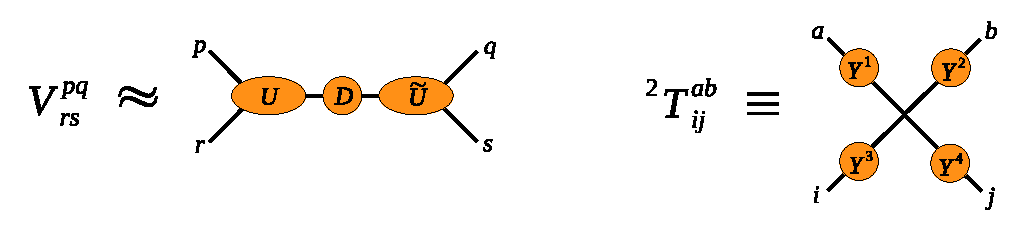
\includegraphics[width=0.9\textwidth]
{figures/cpd_rccsd/rccsd_cpd_def}}}
.
\label{fig:rccsd_cpd_def}
\end{equation}
%
Following the procedure described in Chapter~\ref{ch:tcc}, we derived 
an ALS-like update rule for the factors $Y \in \{Y^{1}, Y^{2}, Y^{3}, Y^{4}\}$. 
We call this method CPD-RCCSD. 
After defining proper intermediates with an automated algebraic 
system,\cite{drudge2} the cost of iteration in CPD-RCCSD is quartic in the 
basis size, auxiliary basis size and $r_{T}$.

CP decomposition was applied in the contest of RCCD before by Benedict and 
Auer.\cite{benedict_ccd, benedict_mp2} Although conceptually similar, our 
method significantly differs in the way one solves for the factors $Y$ of 
the ${}^2T$ amplitude and the use of standard RI decomposition of two-electron 
integrals instead of CPD in the mentioned works.

To study the properties of this new method, we apply it here to weakly 
correlated problems used in the evaluation of 
THC-RCCSD,\cite{schutski2017tensor} as well as to weakly correlated Hubbard 
model. 

\subsection{Computational details}
The CPD-RCCSD code is written in Python~\cite{van2007python} on top of the 
PySCF~\cite{sun2017python} electronic structure package. Hartree-Fock 
solutions, as well as two-electron integrals and density fitted integrals were 
provided by PySCF. For molecular systems we used the standard cc-pVDZ basis set 
from the EMSL database,\cite{schuchardt2007basis} along with the cc-pVDZ-jkfit 
for RI decomposition. In the case of the Hubbard 
Hamiltonian~\ref{sec:hubbard_hamiltonian}
the RI decomposition was built analytically.

For simulations of molecules in Table~\ref{tab:energies_cpd_rccsd} CC iterations 
were stopped after energy converged to within $10^{-6}~\mathrm{H}$ or a limit 
of 500 iterations was reached. In the case of Hubbard Hamiltonian we used a 
threshold of $10^{-12}~\mathrm{t}$ for the energy and 2000 iterations.

\subsection{Exact representations of the Hubbard interaction tensor}
To test the properties of CPD-RCCSD, we employed weakly correlated 
Hubbard models (see Section~\ref{sec:hubbard_hamiltonian}). 
The convenience of the Hubbard Hamiltonian is that the two-body interaction term 
in the on-site basis has simple structure. The full 4-index interaction in a 
model with $N$ sites is a diagonal tensor of size $N\times N\times N \times N$, 
having $\eta$ on the diagonal. Exact representations of the Hubbard interaction 
tensor in various forms can be easily built.

The exact RI representation ($V_{pqrs} = 
\eta \sum_{\alpha} U_{pr\alpha} \tilde{U}_{qs\alpha}$) of the Hubbard 
interaction has rank $N$. Tree index RI factors can be chosen to be sparse $N 
\times N \times N$ tensors with elements $U_{ij\alpha} = \tilde{U}_{ij\alpha} 
= \delta_{i}^{\alpha} \delta_{j}^{\alpha} \cdot \sqrt{\eta}$. Likewise, an 
exact THC decomposition ($V_{pqrs} = \eta \sum_{\alpha \beta} W^{1}_{p\alpha} 
W^{2}_{r\alpha} X_{\alpha, \beta} W^{3}_{q\beta} W^{4}_{s\beta}$) has ranks 
equal $N$, and matrices $W \in \{W^{1}, W^{2}, W^{3}, W^{4}, X\}$ are identity 
matrices of size $N \times N$. The scalar $\eta$ can be absorbed into the 
matrix $X$. Finally, an exact CP decomposition ($V_{pqrs} = \eta \sum_{\alpha} 
W^{1}_{p\alpha} W^{2}_{r\alpha} W^{3}_{q\alpha} W^{4}_{s\alpha}$) has rank $N$.
Factor matrices, as previously, are identities. Summarizing, all decompositions 
of the Hamiltonian considered in this work can be built exactly and have low 
ranks. In Hubbard model calculations the approximations, thus, affect only 
cluster amplitudes.

\subsection{CPD-RCCSD in weakly correlated systems}
We first use CPD-RCCSD to calculate energy of the Hubbard model.
The energies of $6$-, $10$-, $14$- and $18$-site periodic Hubbard systems at 
half-filling were calculated at $\eta = 2$.
%
\begin{figure}[!tb]
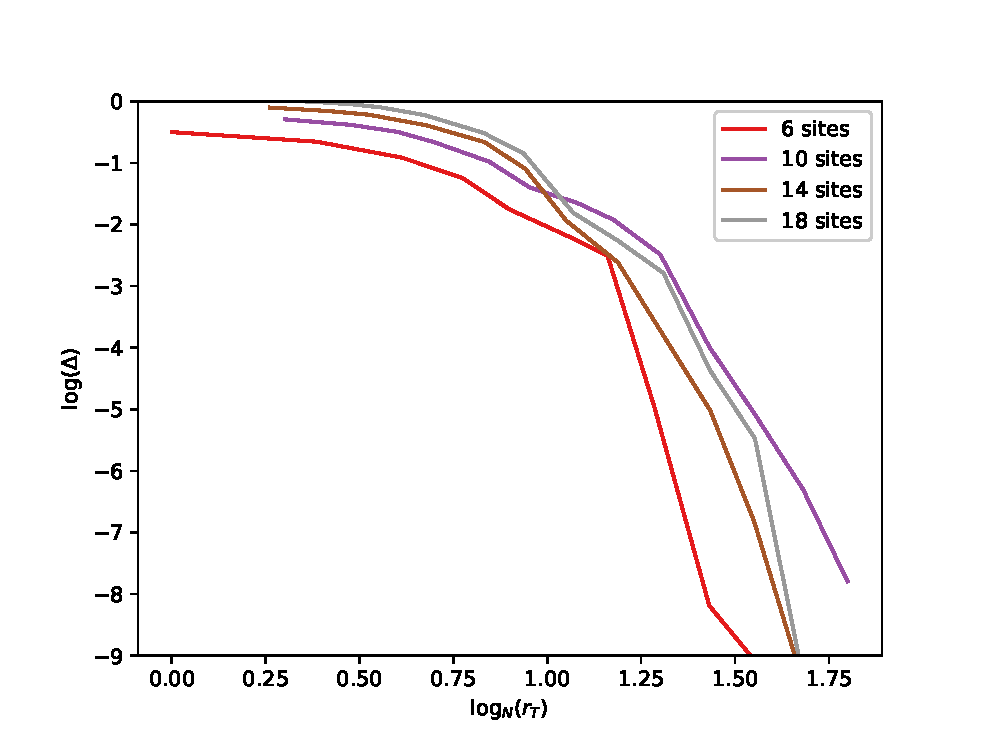
\includegraphics[width=\columnwidth]{figures/cpd_rccsd/err_vs_r_u_2_cpd}
\caption{Absolute error in correlation energy per site for the 
Hubbard model at $\eta = 2$ as the function of rank $r_{T}$ of CP decomposed
${}^2T$ amplitudes, H
\label{fig:err_vs_r_u_2}}
\end{figure}
%
As the graph demonstrates, the difference in the correlation energy 
between CPD-RCCSD and conventional RCCSD methods decays exponentially as the 
rank $r_{T}$ is increased, similarly to the THC-RCCSD method. At  
$r_{T} \sim N^{1.2} - N^{1.5}$ the difference induced by the decomposition 
of doubles amplitudes is less than $10^{-3}~\mathrm{t}$, which an excellent 
approximation of RCCSD. 

To further assess the performance of CPD-RCCSD, we computed the energy 
of a set of molecules previously used for evaluating THC-RCCSD. The magnitude 
of $r_{T}$ is chosen to be a multiple of the size of the auxiliary basis used 
in the RI decomposition of the Hamiltonian.
%
\begin{center}
\begin{table}[!ht]
\caption{CCSD correlation energies ($E_c$), errors in
correlation energies ($\Delta E_c$)
and the norm of doubles residuals ($|{}^2R_{ij}^{ab}|$) for several small 
molecules.
\label{tab:energies_cpd_rccsd}}
\begin{tabular}{lccccccc}
\hline \hline
& & \multicolumn{2}{c}{$\Delta E_c~(mH)$} & 
\multicolumn{2}{c}{$|{}^2R_{ij}^{ab}|$}\\
\cline{3-4} \cline{5-6} System & $E_c~(mH)$ & $1.5 \, N_\mathrm{RI}$ &
$2 \, N_\mathrm{RI}$ & $1.5 \, N_\mathrm{RI}$ &
$2 \,~N_\mathrm{RI}$\\
\hline
AceticAcid & -228.506 & 5.955 & 3.169 & 0.262 & 0.195 \\
Aniline & -286.771 & 14.771 & 7.378 & 0.360 & 0.208 \\
Diboron tetrafluoride & -448.299 & 7.143 & 4.232 & 0.318 & 0.271 \\
Benzene & -231.559 & 11.144 & 5.596 & 0.298 & 0.167 \\
Butadiene & -155.525  & 4.717 & 2.483 & 0.198 & 0.105 \\
Cyclobutane & -156.738  & 5.215 & 2.329 & 0.185 & 0.094 \\
Dimethylsulfoxide & -552.232  & 5.206 & 2.518 & 0.221 & 0.149 \\
Furan & -229.390 & 9.540 & 4.675 & 0.310 & 0.191 \\
Isobutane & -157.973 & 4.187 & 2.242 & 0.124 & 0.087 \\
Methylformate & -228.479 & 6.247 & 3.271 & 0.267 & 0.198 \\
Methylnitrite & -244.398 & 7.112 & 3.856 & 0.290 & 0.209 \\
Pyridine & -247.570 & 11.996 & 6.341 & 0.311 & 0.205 \\
Pyrrole & -209.566 & 9.330 & 4.569 & 0.293 & 0.163 \\
Thiophene & -552.031 & 7.703 & 4.127 & 0.238 & 0.147 \\
Phenol & -306.608 & 14.430 & 7.419 & 0.366 & 0.224 \\
Toluene & -270.758 & 14.333 & 6.706 & 0.355 & 0.171 \\
mean unsigned error & & 8.689 & 4.432 & & &\\
max unsigned error & & 14.771 & 7.419 & & &\\
root-mean-square error& & 9.379 & 4.758 & & &\\
\hline\hline
\end{tabular}
\end{table}
\end{center}
%
The results in Table~\ref{tab:energies_cpd_rccsd} are similar to the results
of THC-RCCSD. As the rank $r_{T}$ is increased, the quality of approximation 
improves. Typical errors are around $5~\mathrm{mH}$ for the rank of CPD of 
doubles amplitudes being twice as large as the size of the auxiliary basis used 
in the decomposition of the Hamiltonian. The errors in CPD-RCCSD are around five 
times higher than in THC-RCCSD for the same rank values. We attribute this to 
the larger number of the parameters in THC-RCCSD, having $4 \cdot N r_{T} + 
r^{2}_{T}$ for parameterizing amplitudes versus $4 \cdot N r_{T}$ in CPD-RCCSD. 
The comparison of Tables~\ref{tab:energies_cpd_rccsd} and 
\ref{tab:energies_cpd_rccsd} shows, however, that the accuracy of CPD-RCCSD 
increases more monotonically with the size of the rank. We suspect that a 
cancellation of errors happens in case of THC-RCCSD because of the more 
complicated approximation to the Hamiltonian, and CPD-based coupled 
cluster provides a more predictable approximation.

\subsection{Conclusions}
To summarize, CPD-RCCSD provides an alternative efficient approximation to the 
coupled cluster with singles and doubles. Overall, CPD-RCCSD and THC-RCCSD 
have a similar accuracy and asymptotic scaling of computational cost. 
Practically, CPD-RCCSD is much faster due to the use of an efficient RI 
decomposition of the electron interaction in place of THC. An additional 
benefit of using canonical decomposition of amplitudes is that the method can 
be further generalized to higher order coupled cluster theories.

